\section{The Disaster Scenario}
%[[Feng]]
\noindent We consider a disaster scenario involving a satellite, containing radioactive fuel, that has crashed in a sub-urban area (see Section \ref{atomic} to see how this helps implement a credible mixed-reality game). While debris is strewn around a large area, damaging buildings and causing accidents and injuring civilians, radioactive discharge from the debris is gradually spreading over the area, threatening to contaminate food reserves and people. Hence, emergency services, voluntary organisations, and the military are deployed to help evacuate the casualties and resources before these are engulfed by  radioactive cloud.  In what follows, we model this scenario formally and then describe the optimisation problem faced by the actors (i.e., including emergency services, volunteers, medics, and soldiers) in trying to save as many lives and resources as they can.

\subsection{Formal Model}
\noindent Let $G$ denote a grid overlaid on top of the disaster space, and the satellite and actors are located at various coordinates $(x,y) \in G$ in this grid. The set of field responders be denoted as $i_1, \cdots, i_n \in I$ and the set of rescue tasks as  $t_1,\cdots, t_m\in T$.  As responders enact tasks, they may become tired or get injured. Hence, we assign each responder  a health level $h_i\in [0,100]$. Moreover, each responder will have  a specific role  $r \in Roles$ (e.g., fire brigade, soldier, or medic) and this will determine the capabilities he or she has and therefore the tasks he or she can perform. We denote as $Roles(i)$ the role of responder $i$. In turn, to complete a given task $t$,  a set of responders $I' \subseteq I$ with specific roles $R_t \subseteq R$ is required. Thus, a task can only be completed by a team of responders $I'$ if $\{Roles(i) | i \in I'\} = R_t$. 

Given this model, we next formulate the optimisation problem faced by the responders (and later solved in Section \ref{sec:algo}). To this end, we propose a Multi-Agent Markov Decision Process that captures XX and XX \textbf{Feng: add justification for MMDP approach and what uncertainties you capture - say how this is different from CFST for example}.

\subsection{Radiation Cloud Modelling}\label{sec:radiation}
\noindent The radiation cloud is assumed to be monitored using a number of sensors on the ground (within the disaster space) that collect readings of the radiation cloud intensity and wind velocity every minute of the game. These sensors can be at fixed locations or held by mobile agents.  The radiation cloud diffusion process is modelled in a standard way by a nonlinear Markov field stochastic differential equation,  
\begin{eqnarray*}
\frac{D \text{Rad}({\bf z}, \tau)}{D \tau}=\kappa \triangledown^2 \text{Rad}({\bf z},\tau)-\text{Rad}({\bf z},\tau)\triangledown \cdot {\bf w}({\bf z},\tau)+\sigma({\bf z},\tau)
\end{eqnarray*}
where $D$ is the material derivative, $\text{Rad}({\bf z},\tau)$ is the radiation cloud intensity at location ${\bf z}$ at time $\tau$, $\kappa$ is a fixed diffusion coefficient and $\sigma$ is the radiation source(s) emission rate. The diffusion equation is solved on a regular grid defined across the environment with grid coordinates $G$ (as defined in Section \ref{sec:model}).  Furthermore, the grid is solved at discrete time instances $\tau$.  The cloud is driven by wind forces which vary both spatially and temporally.  These forces induce anisotropy into the cloud diffusion process which is proportional to the wind velocity, ${\bf w}({\bf z},\tau)$.  The wind velocity is drawn from two independent Gaussian processes (GP), one GP for each Cartesian coordinate axis, $w_i({\bf z},\tau)$, of ${\bf w}({\bf z},\tau)$.  The GP captures both the spatial distribution of the wind velocity and the dynamic process resulting from shifting wind patterns such as short term gusts and longer term variations. 

% In our simulation, each spatial wind velocity component is modelled by a squared-exponential GP covariance function, $K$, with fixed input and output scales (although any covariance function can be substituted). Furthermore, as wind conditions may change over time we introduce a temporal correlation coefficient, $\rho$, to the covariance function.  Thus, for a single component, $w_i$, of ${\bf w}$, defined over grid $G$ at times $\tau$ and $\tau^\prime$, the wind process covariance function is, $\text{Cov}(w_i(G,\tau),w_i(G,\tau^\prime))=\rho(\tau,\tau^\prime) K(G,G)$.  We note that, when $\rho=1$ the wind velocities are time invariant (although spatially variant).  Values of $\rho<1$ model wind conditions that change over time.

Using the above model, we are able to create a moving radiation cloud, thus posing a real challenge both for the HQ (agent and commander) and the responders on the ground, as predictions they can make of where the cloud will move to will be prone to uncertainty both to the simulated wind speed and direction. 


%(\textbf{Steve: in the platform we take the `real' values from the diffusion process i believe. Does the above capture this? We will say that we will add the features you mention below to a future version of the platform where we aim to do both situational awareness and rescue. Add a sentence above to conclude where we took the values from and the process takes into account the  location of radiation source. Also, your notation clashes with the notations in the scenario and Feng's algorithm - please try to align.}
%The cloud intensity and wind velocity are measured by {\it monitor agents} equipped with geiger-counters and anemometers.  These agents are directed to take measurements with greatest information gain in the radiation cloud intensity.  The measurements are folded into the EKF and this refines estimates of the radiation cloud across the grid.  Figure~\ref{radiation_screen_shots} shows example cloud simulations for slow varying (i.e. $\rho=0.99$) and gusty (i.e. $\rho=0.90$) wind conditions.  Figure~\ref{radiation_screen_shots}(a) shows slow varying wind conditions in which case the radiation cloud can be interpolated accurately using sparse sensor measurements and the LFM model.  Alternatively, during gusty conditions the radiation cloud model is more uncertain far from the locations where recent measurements have been taken, as shown in Figure~\ref{radiation_screen_shots}(b).
%
%\begin{figure}[ht] \begin{center}
%    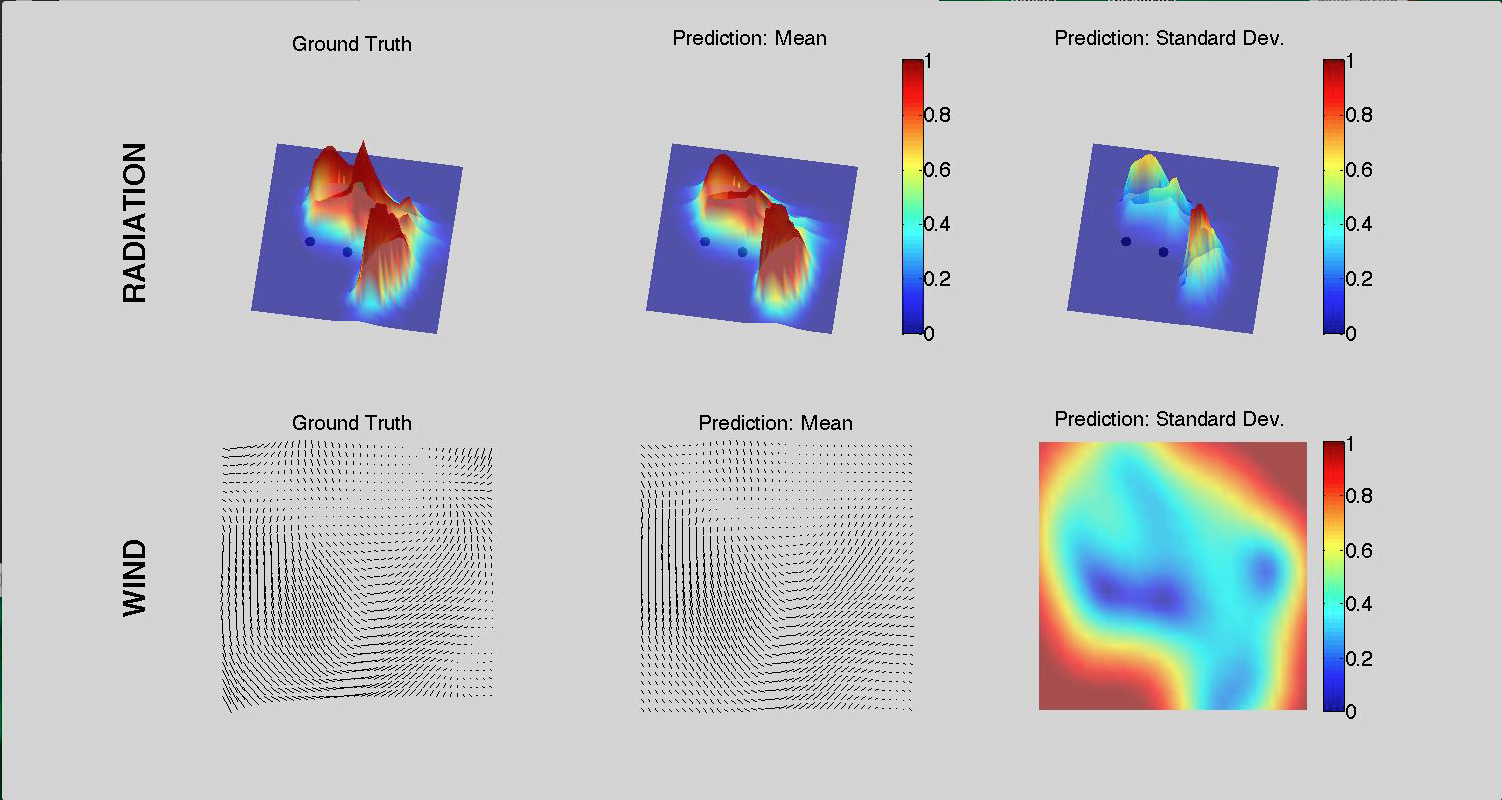
\includegraphics[width=0.45\textwidth]{figures/radiation_ss_calm.png}\\
%    (a) Slowly varying wind conditions\\ \ \\
%    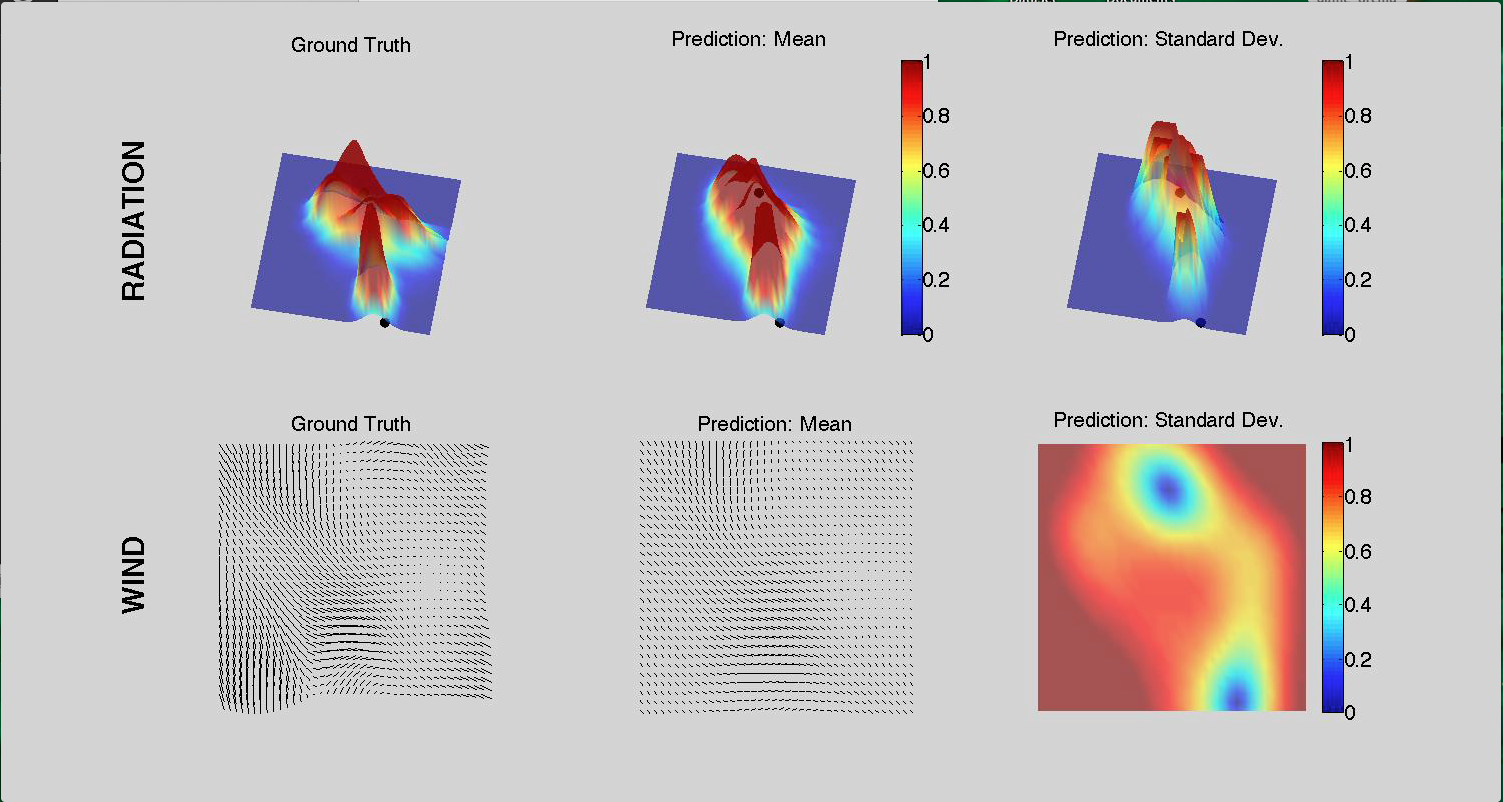
\includegraphics[width=0.45\textwidth]{figures/radiation_ss_gust.png}\\
%    (b) Gusty wind conditions 
%\caption{\label{radiation_screen_shots} Radiation and wind simulation ground truth and EKF estimates obtained using measurements from monitor agents (black dots).  Left most panes are ground truth radiation and wind conditions, the middle panes are corresponding estimates and right most panes are state uncertainties:  (a) Invariant and (b) gusty wind conditions.}
%\end{center}
%\end{figure}

\subsection{The Optimisation Problem}
 Markov decision process (MMDP),
$\langle I, S, \{A_i\}, P, R \rangle$, where:
\begin{itemize}
  \item $I$ is a set of $n$ game players. 
  \item $S = S_r \times S_{p_1} \times \cdots \times S_{p_n}
      \times S_{t_1} \times \cdots \times S_{t_m}$ is the state
      space: $S_r$ is the state variable of the radiation cloud
      to specify the radiation level (between 0 and 100) of
      each grid; $S_{p_i}$ is the state variable for player $i$
      to specify his current health level and location;
      $S_{t_j}$ is the state variable for task $j$ to specify
      its status (picked up, dropped off, or idle) and
      location.
  \item $A_i$ is a set of player $i$'s actions. Each player can
      stay in his current grid, move to his 8 neighboring grids
      (N, NE, E, SE, S, SW, W, NW), or pickup/drop a task
      located in his current grid. A joint action is a list of
      actions, $\vec{a}=\langle a_1, \cdots, a_n \rangle$, one
      for each player.
  \item $P = P_r \times P_{p_1} \times P_{p_n} \times P_{t_1}
      \times P_{t_n}$ is the transition function:
      $P_r(s'_r|s_r)$ is the probability for the radiation
      cloud to expand from state variable $s_r$ to $s'_r$;
      $P_{p_i}(s'_{p_i}|s_{p_i}, a_i)$ is the probability for
      player $i$ to transit from state variable $s_{p_i}$ to
      $s'_{p_i}$ when executing action $a_i$ (e.g., when a
      player moves to north, his health level and location will
      be updated based on his previous health level and
      location); $P_{t_j}(s'_{t_j}|s_{t_j}, \vec{a})$ is the
      transition probability for task $j$ and a task transits
      to a new state only when all the necessarily skilled
      players are located in the same grid as the task and
      perform the ``pickup/drop" actions at the same time.
  \item $R$ is the reward function. If a task has been dropped
      off on any dropoff zone, a big reward is received. A huge
      penalty is given if a player is killed. Each player's
      action is associated with a small cost.
\end{itemize}
At each time step of the game, we assume the planning agent is
fully observable of the current state. Thus, a plan (a.k.a policy)
for the team is a mapping from states to joint actions, $\pi: S
\rightarrow \vec{A}$. By given a plan, the players know how to act
in the field. The expected value of a plan $\pi$ can be computed
recursively by the Bellman equation:
\begin{equation}
  V^\pi(s) = R(s, \pi(s)) + \gamma \sum_{s'\in S} P(s'|s, \pi(s)) V^\pi(s')
\end{equation}
where $\pi(s)$ is a joint action selected by the plan and $\gamma
\in (0, 1]$ is the discount factor. The goal of solving the game is
to find an optimal plan $\pi^*$ that maximize the expected value
given the initial state $s^0$, $\pi^* = \arg\max_{\pi} V^\pi(s^0)$.
